% !TEX TS-program = pdflatex
\documentclass[11pt]{article}

% -------------------- Packages --------------------
\usepackage[a4paper,margin=1in]{geometry}
\usepackage{amsmath,amssymb}
\usepackage[T1]{fontenc}
\usepackage{lmodern}
\usepackage{xcolor}
\usepackage{tcolorbox}
\tcbuselibrary{skins,breakable}
\usepackage{enumitem}
\usepackage{hyperref}
\usepackage{tikz}
\usetikzlibrary{calc,angles,quotes,arrows.meta,matrix,positioning}
\usepackage{graphicx} % for \resizebox

\pagestyle{empty}

% -------------------- Dark Theme Colors --------------------
\definecolor{bg}{HTML}{000000}
\definecolor{pairbg}{HTML}{121212}
\definecolor{solbg}{HTML}{0A0A0A}
\definecolor{border}{HTML}{2A2A2A}
\definecolor{text}{HTML}{FFFFFF}
\definecolor{muted}{HTML}{C9CDD3}
\definecolor{gold}{HTML}{FFD700}
\definecolor{green}{HTML}{4ADE80}
\definecolor{cyan}{HTML}{38BDF8}

\pagecolor{bg}
\color{text}

\hypersetup{
  colorlinks=true,
  linkcolor=cyan,
  urlcolor=cyan
}

\setlength{\parindent}{0pt}
\setlength{\parskip}{10pt}

% Help LaTeX avoid overfull lines globally (text mode)
\sloppy
\setlength{\emergencystretch}{3em}

\setlist[itemize]{left=1.4em,itemsep=6pt,topsep=6pt}
\setlist[enumerate]{left=1.6em,itemsep=4pt,topsep=4pt}

% -------------------- tcolorbox Base --------------------
\tcbset{
  enhanced,
  breakable,
  arc=12pt,
  boxrule=0.8pt,
  left=14pt,right=14pt,top=12pt,bottom=12pt
}

\newtcolorbox{QAPair}[1]{%
  colback=pairbg,
  colbacklower=solbg,
  colframe=border,
  coltext=text,
  title=\textcolor{gold}{\bfseries #1},
  fonttitle=\bfseries,
  coltitle=text,
  segmentation style={draw=border, dashed, line width=0.6pt},
  before upper=\raggedright,
  before lower=\raggedright
}

\newtcolorbox{QuickBox}{%
  colback=pairbg,
  colframe=cyan,
  coltext=text,
  fontupper=\color{text}\raggedright,
  borderline north={4pt}{0pt}{cyan},
  arc=14pt,
  boxrule=0.8pt
}

% Helper for step headings
\newcommand{\Step}[1]{\textcolor{muted}{\textbf{Step #1:}}}

% ------------------------------------------------------------
% StepDiagram: auto-scale diagrams ONLY if too wide (prevents right overflow)
% ------------------------------------------------------------
\newsavebox{\StepBox}
\newenvironment{StepDiagram}{%
  \par\medskip
  \begin{center}
  \begin{lrbox}{\StepBox}\begin{minipage}{\linewidth}\centering
}{%
  \end{minipage}\end{lrbox}%
  \ifdim\wd\StepBox>\linewidth
    \resizebox{\linewidth}{!}{\usebox{\StepBox}}%
  \else
    \usebox{\StepBox}%
  \fi
  \end{center}
  \medskip
}

% TikZ styles
\tikzset{
  base/.style={draw=text, line width=0.9pt, line cap=round, line join=round},
  new/.style={draw=cyan, line width=1.2pt, line cap=round, line join=round},
  help/.style={draw=muted, dashed, line width=0.9pt},
  ang/.style={draw=gold, line width=1.0pt},
  dot/.style={circle, fill=text, inner sep=1.2pt},
  lab/.style={text=text, font=\small},
  labm/.style={text=muted, font=\small},
}

% A compact explanation box that WRAPS (safe for long math)
\newcommand{\EqDiagram}[1]{%
\begin{StepDiagram}
\begin{tikzpicture}
\node[
  draw=border,
  rounded corners=10pt,
  inner sep=8pt,
  text=text,
  align=left,
  text width=0.92\linewidth
] {%
\begin{minipage}{0.92\linewidth}\raggedright
#1
\end{minipage}
};
\end{tikzpicture}
\end{StepDiagram}
}

% ============================================================
\begin{document}

\begin{center}
{\LARGE\bfseries \textcolor{gold}{Exercise 12.1 --- Solutions}}\\[-2pt]
\end{center}

% -------------------- Quick formulas + diagram PER LINE --------------------
\begin{QuickBox}
{\color{cyan}\bfseries Quick formulas (Cumulative Frequency, Ogive, Quartiles \& Percentiles)}\par\medskip

\begin{itemize}
\item \textbf{Less-than cumulative frequency:}
\[
CF_k=f_1+f_2+\cdots+f_k.
\]
\begin{StepDiagram}
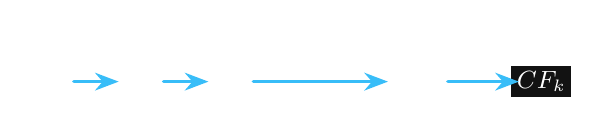
\begin{tikzpicture}[scale=0.95]
\node[lab] at (-3.2,0.65) {$f_1$};
\node[lab] at (-2.0,0.65) {$f_2$};
\node[lab] at (-0.8,0.65) {$f_3$};
\node[lab] at ( 0.4,0.65) {$\cdots$};
\node[lab] at ( 1.6,0.65) {$f_k$};

\draw[base, rounded corners=6pt] (-3.5,0) rectangle (-2.9,0.4);
\draw[base, rounded corners=6pt] (-2.3,0) rectangle (-1.7,0.4);
\draw[base, rounded corners=6pt] (-1.1,0) rectangle (-0.5,0.4);
\draw[base, rounded corners=6pt] ( 1.3,0) rectangle ( 1.9,0.4);

\draw[new, -{Stealth[length=3mm]}] (-2.9,0.2) -- (-2.3,0.2);
\draw[new, -{Stealth[length=3mm]}] (-1.7,0.2) -- (-1.1,0.2);
\draw[new, -{Stealth[length=3mm]}] (-0.5,0.2) -- ( 1.3,0.2);

\node[lab, fill=pairbg, inner sep=2pt] at (3.35,0.2) {$CF_k$};
\draw[new, -{Stealth[length=3mm]}] (2.1,0.2) -- (3.05,0.2);
\end{tikzpicture}
\end{StepDiagram}

\item \textbf{Class boundaries (for inclusive integer classes):}
If class is $a$--$b$, then boundaries are $(a-0.5)$ to $(b+0.5)$.
\begin{StepDiagram}
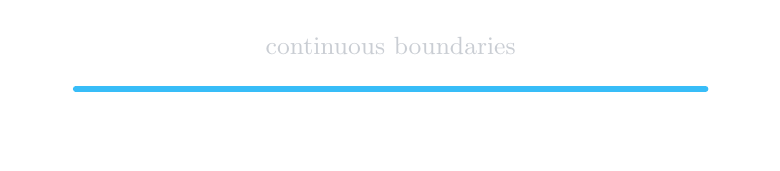
\begin{tikzpicture}[scale=1.0]
\draw[base, -{Stealth[length=3mm]}] (-0.2,0) -- (8.4,0);
\foreach \x/\t in {0/{$a-0.5$},3/{$a$},6/{$b$},8/{$b+0.5$}}{
  \draw[base] (\x,0.12)--(\x,-0.12);
  \node[lab] at (\x,-0.45) {\t};
}
\draw[new, line width=2pt] (0,0) -- (8,0);
\node[labm] at (4,0.55) {continuous boundaries};
\end{tikzpicture}
\end{StepDiagram}

\item \textbf{Grouped-data formula (quartile/decile/percentile):}
\[
\text{Value}=L+\Big(\frac{(pN)-CF_{\text{prev}}}{f}\Big)\,h,
\qquad p=\frac14,\frac{7}{10},\frac{30}{100},\dots
\]
\begin{StepDiagram}
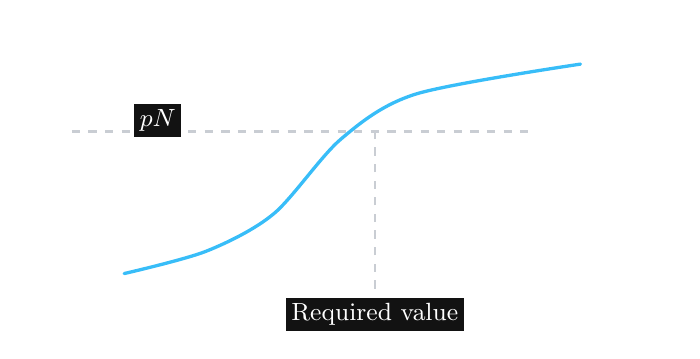
\begin{tikzpicture}[scale=0.95]
\draw[base, -{Stealth[length=3mm]}] (0,0) -- (7.6,0);
\draw[base, -{Stealth[length=3mm]}] (0,0) -- (0,3.2);
\node[lab] at (7.8,-0.15) {$x$};
\node[lab] at (-0.2,3.25) {$CF$};

\draw[new] plot[smooth] coordinates {(0.7,0.2) (1.8,0.5) (2.7,1.0) (3.6,2.0) (4.6,2.6) (6.8,3.0)};
\draw[help] (0,2.1) -- (6.2,2.1);
\draw[help] (4.05,0) -- (4.05,2.1);
\node[lab, fill=pairbg, inner sep=2pt] at (1.15,2.25) {$pN$};
\node[lab, fill=pairbg, inner sep=2pt] at (4.05,-0.35) {Required value};
\end{tikzpicture}
\end{StepDiagram}

\item \textbf{Median is the 50th percentile:}
\[
\text{Median}=L+\Big(\frac{\frac{N}{2}-CF_{\text{prev}}}{f}\Big)\,h.
\]
\begin{StepDiagram}
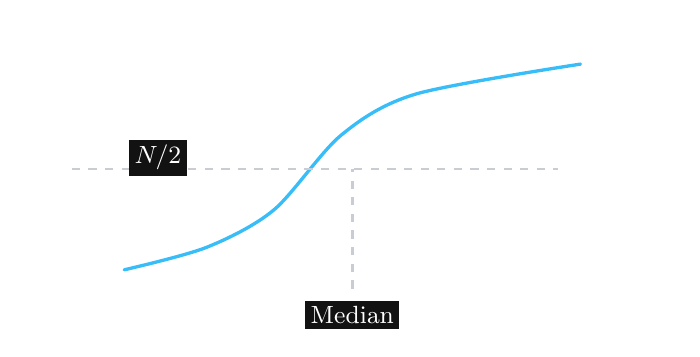
\begin{tikzpicture}[scale=0.95]
\draw[base, -{Stealth[length=3mm]}] (0,0) -- (7.6,0);
\draw[base, -{Stealth[length=3mm]}] (0,0) -- (0,3.2);
\node[lab] at (7.8,-0.15) {$x$};
\node[lab] at (-0.2,3.25) {$CF$};

\draw[new] plot[smooth] coordinates {(0.7,0.25) (1.8,0.55) (2.7,1.05) (3.6,2.05) (4.6,2.6) (6.8,3.0)};
\draw[help] (0,1.6) -- (6.5,1.6);
\draw[help] (3.75,0) -- (3.75,1.6);
\node[lab, fill=pairbg, inner sep=2pt] at (1.15,1.75) {$N/2$};
\node[lab, fill=pairbg, inner sep=2pt] at (3.75,-0.35) {Median};
\end{tikzpicture}
\end{StepDiagram}

\item \textbf{Items above a value $x$:}
\[
\#(>x)=N-CF(x).
\]
\begin{StepDiagram}
\begin{tikzpicture}[scale=0.95]
\draw[base, -{Stealth[length=3mm]}] (0,0) -- (7.6,0);
\draw[base, -{Stealth[length=3mm]}] (0,0) -- (0,3.2);
\node[lab] at (7.8,-0.15) {$x$};
\node[lab] at (-0.2,3.25) {$CF$};

\draw[new] plot[smooth] coordinates {(0.7,0.25) (1.8,0.55) (2.7,1.05) (3.6,2.05) (4.6,2.6) (6.8,3.0)};
\draw[help] (4.3,0) -- (4.3,2.3);
\node[lab, fill=pairbg, inner sep=2pt] at (4.3,-0.35) {$x$};
\node[labm] at (5.95,2.65) {portion above $x$};
\end{tikzpicture}
\end{StepDiagram}

\item \textbf{Range:}
\[
\text{Range}=\text{Max}-\text{Min}.
\]
\begin{StepDiagram}
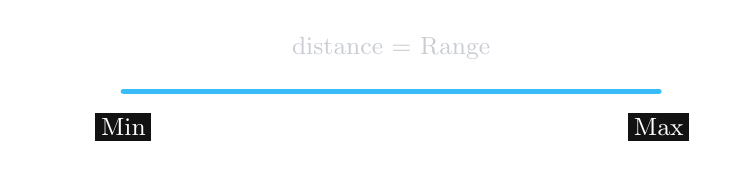
\begin{tikzpicture}[scale=1.0]
\draw[base, -{Stealth[length=3mm]}] (-0.2,0) -- (8.6,0);
\draw[new, line width=2pt] (1.0,0) -- (7.8,0);
\node[lab, fill=pairbg, inner sep=2pt] at (1.0,-0.45) {Min};
\node[lab, fill=pairbg, inner sep=2pt] at (7.8,-0.45) {Max};
\node[labm] at (4.4,0.55) {distance = Range};
\end{tikzpicture}
\end{StepDiagram}

\item \textbf{Interquartile Range (IQR):}
\[
IQR=Q_3-Q_1.
\]
\begin{StepDiagram}

\begin{tikzpicture}[scale=1.0]
\draw[base, -{Stealth[length=3mm]}] (-0.2,0) -- (9.2,0);
\foreach \x/\t in {1/{$Q_1$},4.5/{$Q_2$},8/{$Q_3$}}{
  \draw[base] (\x,0.12)--(\x,-0.12);
  \node[lab] at (\x,-0.45) {\t};
}
\draw[new, line width=2pt] (1,0) -- (8,0);
\node[labm] at (4.5,0.55) {IQR span};
\end{tikzpicture}
\end{StepDiagram}

\item \textbf{Quartile positions:}
\[
Q_1=P_{25},\quad Q_2=P_{50}(\text{median}),\quad Q_3=P_{75},\qquad D_7=P_{70}.
\]
\begin{StepDiagram}

\begin{tikzpicture}[scale=1.0]
\draw[base] (0,0) rectangle (8,0.8);
\draw[new] (0,0) rectangle (2,0.8);
\draw[new] (2,0) rectangle (4,0.8);
\draw[new] (4,0) rectangle (6,0.8);
\draw[new] (6,0) rectangle (8,0.8);
\node[lab] at (1,0.4) {$25\%$};
\node[lab] at (3,0.4) {$25\%$};
\node[lab] at (5,0.4) {$25\%$};
\node[lab] at (7,0.4) {$25\%$};
\node[labm] at (2,-0.35) {$Q_1$};
\node[labm] at (4,-0.35) {$Q_2$};
\node[labm] at (6,-0.35) {$Q_3$};
\end{tikzpicture}
\end{StepDiagram}

\end{itemize}
\end{QuickBox}

% ============================================================
% Q1
\begin{QAPair}{Question 1}
\textcolor{gold}{\bfseries Question:} Construct cumulative frequency column for the frequency table and answer:
(i) total items, (ii) class interval of 8th item, (iii) items having worth $<21$,
(iv) group with highest items, (v) lower boundary of last class.

\[
\begin{array}{c|cccccc}
\text{Class interval} & 1\!-\!10 & 11\!-\!20 & 21\!-\!30 & 31\!-\!40 & 41\!-\!50 & 51\!-\!60\\ \hline
f & 3 & 4 & 7 & 9 & 5 & 2
\end{array}
\]
\tcblower
\textcolor{green}{\bfseries Answer:}\par

\Step{1} Make the less-than cumulative frequency (running total).
\begin{StepDiagram}
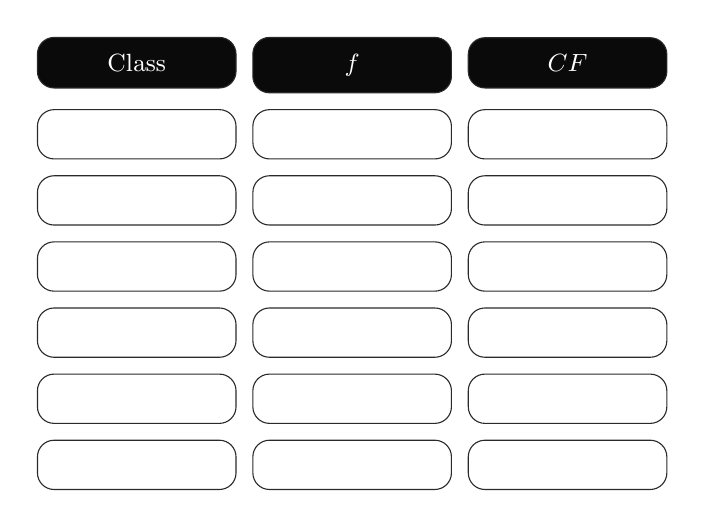
\begin{tikzpicture}
\matrix[matrix of nodes,
  nodes={draw=border, rounded corners=6pt, text width=2.1cm, align=center, font=\small, text=text, inner sep=6pt},
  row sep=2mm, column sep=2mm] (m) {
|[fill=solbg]| Class & |[fill=solbg]| $f$ & |[fill=solbg]| $CF$ \\
$1$--$10$ & $3$ & $3$ \\
$11$--$20$ & $4$ & $7$ \\
$21$--$30$ & $7$ & $14$ \\
$31$--$40$ & $9$ & $23$ \\
$41$--$50$ & $5$ & $28$ \\
$51$--$60$ & $2$ & $30$ \\
};
\end{tikzpicture}
\end{StepDiagram}

\Step{2} Total number of items is the last cumulative frequency.
\EqDiagram{\(\displaystyle N=30\) (last cumulative frequency)}

\Step{3} The 8th item lies where cumulative frequency first becomes \(\ge 8\):
\[
CF=7 \text{ up to }20,\quad CF=14 \text{ up to }30 \Rightarrow \text{8th item in } 21\text{--}30.
\]
\begin{StepDiagram}
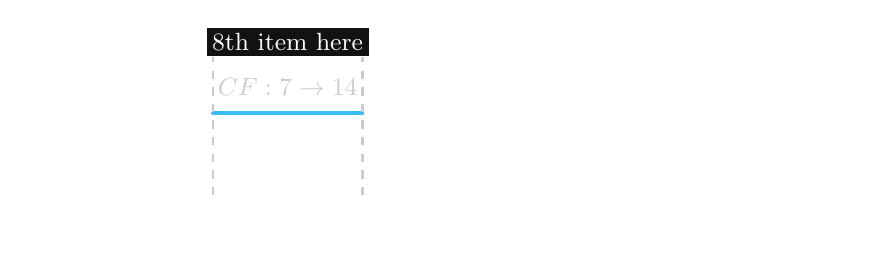
\begin{tikzpicture}[scale=0.95]
\draw[base, -{Stealth[length=3mm]}] (0,0) -- (10.2,0);
\foreach \x/\t in {0/{$\le10$},2/{$\le20$},4/{$\le30$},6/{$\le40$},8/{$\le50$},10/{$\le60$}}{
  \draw[base] (\x,0.12)--(\x,-0.12);
  \node[lab] at (\x,-0.45) {\t};
}
\draw[new] (2,1.1) -- (4,1.1);
\node[labm] at (3,1.45) {$CF:7\to 14$};

\draw[help] (2,0.0) -- (2,1.85);
\draw[help] (4,0.0) -- (4,1.85);
\node[lab, fill=pairbg, inner sep=2pt] at (3,2.05) {8th item here};
\end{tikzpicture}
\end{StepDiagram}

\Step{4} Items having worth \(<21\) means values up to \(20\Rightarrow CF\) at \(11\text{--}20\).
\EqDiagram{\(\displaystyle \#(<21)=CF(\le 20)=7\)}

\Step{5} The highest frequency is \(9\) in class \(31\text{--}40\).
\begin{StepDiagram}
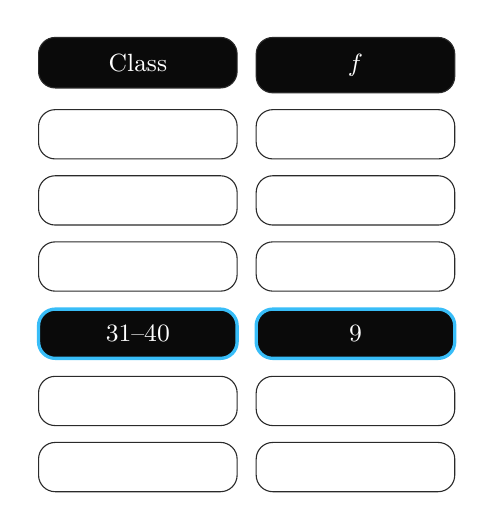
\begin{tikzpicture}
\matrix[matrix of nodes,
  nodes={draw=border, rounded corners=6pt, text width=2.1cm, align=center, font=\small, text=text, inner sep=6pt},
  row sep=2mm, column sep=2mm] (m) {
|[fill=solbg]| Class & |[fill=solbg]| $f$ \\
$1$--$10$ & $3$ \\
$11$--$20$ & $4$ \\
$21$--$30$ & $7$ \\
|[draw=cyan, fill=solbg, line width=1.2pt]| $31$--$40$ & |[draw=cyan, fill=solbg, line width=1.2pt]| $9$ \\
$41$--$50$ & $5$ \\
$51$--$60$ & $2$ \\
};
\end{tikzpicture}
\end{StepDiagram}

\Step{6} Lower boundary of the last class \(51\text{--}60\) is \(50.5\).
\begin{StepDiagram}

\begin{tikzpicture}[scale=1.0]
\draw[base, -{Stealth[length=3mm]}] (-0.2,0) -- (8.2,0);
\draw[base] (1.2,0.12)--(1.2,-0.12);
\draw[base] (6.6,0.12)--(6.6,-0.12);
\node[lab] at (1.2,-0.45) {$50.5$};
\node[lab] at (6.6,-0.45) {$60.5$};
\draw[new, line width=2pt] (1.2,0) -- (6.6,0);
\node[labm] at (3.9,0.55) {boundaries of $51$--$60$};
\end{tikzpicture}
\end{StepDiagram}

\[
\boxed{
\begin{aligned}
&\text{(i) }N=30,\quad
\text{(ii) }21\text{--}30,\quad
\text{(iii) }7,\\
&\text{(iv) }31\text{--}40,\quad
\text{(v) lower boundary}=50.5
\end{aligned}}
\]
\end{QAPair}

% ============================================================
% Q2
\begin{QAPair}{Question 2}
\textcolor{gold}{\bfseries Question:} The mass gained by a new born baby is:

\[
\begin{array}{c|cccccc}
\text{Age (months)} & 1&2&3&4&5&6\\ \hline
\text{kg gained} & 4&3&2&3&2&1
\end{array}
\]

Draw a cumulative frequency polygon (not ogive) and from the graph estimate how much he/she weighed at age \(4.5\) months.
\tcblower
\textcolor{green}{\bfseries Answer:}\par

\Step{1} Convert to cumulative mass gained (running total).
\begin{StepDiagram}
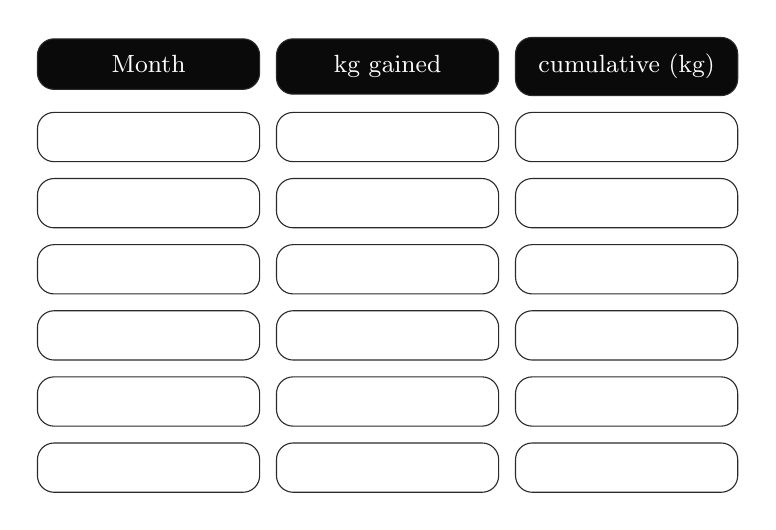
\begin{tikzpicture}
\matrix[matrix of nodes,
  nodes={draw=border, rounded corners=6pt, text width=2.4cm, align=center, font=\small, text=text, inner sep=6pt},
  row sep=2mm, column sep=2mm] (m) {
|[fill=solbg]| Month & |[fill=solbg]| kg gained & |[fill=solbg]| cumulative (kg) \\
$1$ & $4$ & $4$ \\
$2$ & $3$ & $7$ \\
$3$ & $2$ & $9$ \\
$4$ & $3$ & $12$ \\
$5$ & $2$ & $14$ \\
$6$ & $1$ & $15$ \\
};
\end{tikzpicture}
\end{StepDiagram}

\Step{2} Plot points and join them (cumulative frequency polygon).
\begin{StepDiagram}
\begin{tikzpicture}[scale=0.95]
\draw[base, -{Stealth[length=3mm]}] (0,0) -- (8.2,0);
\draw[base, -{Stealth[length=3mm]}] (0,0) -- (0,5.4);
\node[lab] at (8.35,-0.15) {Age (months)};
\node[lab] at (-0.25,5.5) {Cumulative kg};

% x ticks (1..6)
\foreach \x/\t in {1/1,2/2,3/3,4/4,5/5,6/6}{
  \draw[base] (\x,0.12)--(\x,-0.12);
  \node[lab] at (\x,-0.45) {\t};
}
% y ticks (scaled by /3)
\foreach \y/\t in {1/3,2/6,3/9,4/12,5/15}{
  \draw[base] (0.12,\y)--(-0.12,\y);
  \node[lab] at (-0.45,\y) {\t};
}

\coordinate (P1) at (1,1.33);
\coordinate (P2) at (2,2.33);
\coordinate (P3) at (3,3.00);
\coordinate (P4) at (4,4.00);
\coordinate (P5) at (5,4.67);
\coordinate (P6) at (6,5.00);

\draw[new] (P1)--(P2)--(P3)--(P4)--(P5)--(P6);
\foreach \p in {P1,P2,P3,P4,P5,P6}{\node[dot] at (\p) {};}

\node[labm] at (4.3,5.25) {joined points = polygon};
\end{tikzpicture}
\end{StepDiagram}

\Step{3} Read value at \(4.5\) months (linear interpolation between months 4 and 5).
\EqDiagram{%
\[
\begin{aligned}
(4,12)\ \text{to}\ (5,14)\quad &\Rightarrow\quad 4.5\ \text{is the midpoint}\\
\text{so } \; 12+\tfrac12(14-12) &= 13.
\end{aligned}
\]
}

\begin{StepDiagram}
\begin{tikzpicture}[scale=0.95]
\draw[base, -{Stealth[length=3mm]}] (0,0) -- (8.2,0);
\draw[base, -{Stealth[length=3mm]}] (0,0) -- (0,5.4);

\foreach \x/\t in {4/4,5/5}{
  \draw[base] (\x,0.12)--(\x,-0.12);
  \node[lab] at (\x,-0.45) {\t};
}
\foreach \y/\t in {4/12,4.67/14}{
  \draw[base] (0.12,\y)--(-0.12,\y);
  \node[lab] at (-0.55,\y) {\t};
}

\coordinate (A) at (4,4.0);
\coordinate (B) at (5,4.67);
\draw[new] (A)--(B);
\node[dot] at (A) {};
\node[dot] at (B) {};

\draw[help] (4.5,0) -- (4.5,4.335);
\coordinate (M) at (4.5,4.335);
\node[dot] at (M) {};
\node[lab, fill=pairbg, inner sep=2pt] at (6.15,4.335) {$\approx 13$ kg};

\node[labm] at (6.05,0.6) {at $4.5$ months};
\end{tikzpicture}
\end{StepDiagram}

\[
\boxed{\text{At }4.5\text{ months, cumulative mass gained }\approx 13\text{ kg.}}
\]
\end{QAPair}

% ============================================================
% Q3
\begin{QAPair}{Question 3}
\textcolor{gold}{\bfseries Question:} Ages of refugees in Ghaza camp:

\[
\begin{array}{c|cccccc}
\text{Ages (years)} & 20\!-\!24 & 25\!-\!29 & 30\!-\!34 & 35\!-\!39 & 40\!-\!44 & 45\!-\!49\\ \hline
f & 5 & 16 & 12 & 10 & 8 & 4
\end{array}
\]

Draw an ogive (not polygon) and find: (a) first quartile, (b) 7th decile, (c) 60th percentile.
\tcblower
\textcolor{green}{\bfseries Answer:}\par

\Step{1} Total and cumulative frequencies.
\EqDiagram{\(\displaystyle N=5+16+12+10+8+4=55\)}

\begin{StepDiagram}
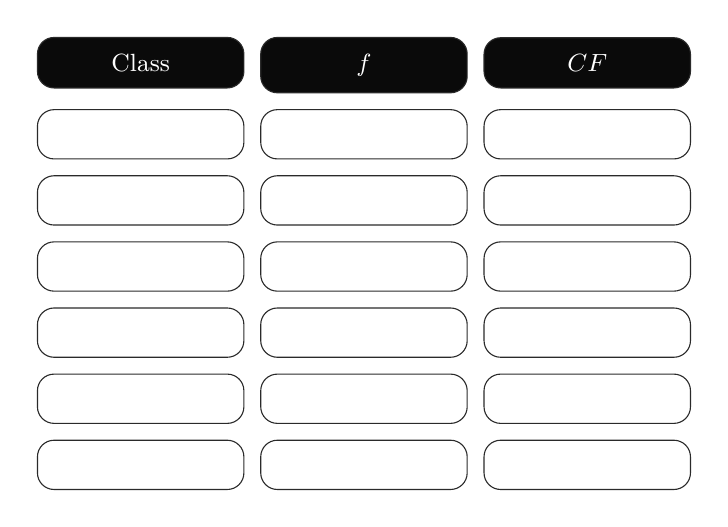
\begin{tikzpicture}
\matrix[matrix of nodes,
  nodes={draw=border, rounded corners=6pt, text width=2.2cm, align=center, font=\small, text=text, inner sep=6pt},
  row sep=2mm, column sep=2mm] (m) {
|[fill=solbg]| Class & |[fill=solbg]| $f$ & |[fill=solbg]| $CF$ \\
$20$--$24$ & $5$ & $5$ \\
$25$--$29$ & $16$ & $21$ \\
$30$--$34$ & $12$ & $33$ \\
$35$--$39$ & $10$ & $43$ \\
$40$--$44$ & $8$ & $51$ \\
$45$--$49$ & $4$ & $55$ \\
};
\end{tikzpicture}
\end{StepDiagram}

\Step{2} Use class boundaries and plot ogive points (upper boundary vs \(CF\)).
Boundaries: \(24.5, 29.5, 34.5, 39.5, 44.5, 49.5\) (class width \(h=5\)).

\begin{StepDiagram}
\begin{tikzpicture}[scale=0.95]
\draw[base, -{Stealth[length=3mm]}] (0,0) -- (8.6,0);
\draw[base, -{Stealth[length=3mm]}] (0,0) -- (0,6.2);
\node[lab] at (8.75,-0.15) {Upper boundary};
\node[lab] at (-0.25,6.35) {CF};

% x ticks (24.5..49.5 mapped 1..6)
\foreach \x/\t in {1/24.5,2/29.5,3/34.5,4/39.5,5/44.5,6/49.5}{
  \draw[base] (\x,0.12)--(\x,-0.12);
  \node[lab] at (\x,-0.45) {\t};
}
% y ticks (5..55 mapped by /10)
\foreach \y/\t in {0.5/5,2.1/21,3.3/33,4.3/43,5.1/51,5.5/55}{
  \draw[base] (0.12,\y)--(-0.12,\y);
  \node[lab] at (-0.75,\y) {\t};
}

\coordinate (A) at (1,0.5);
\coordinate (B) at (2,2.1);
\coordinate (C) at (3,3.3);
\coordinate (D) at (4,4.3);
\coordinate (E) at (5,5.1);
\coordinate (F) at (6,5.5);

\draw[new] (A)--(B)--(C)--(D)--(E)--(F);
\foreach \p in {A,B,C,D,E,F}{\node[dot] at (\p) {};}
\node[labm] at (4.8,5.95) {ogive (schematic)};
\end{tikzpicture}
\end{StepDiagram}

\Step{3} First quartile: position \(N/4=55/4=13.75\) lies in class \(25\text{--}29\).
\EqDiagram{%
\[
\begin{aligned}
Q_1 &= L+\Big(\frac{13.75-CF_{\text{prev}}}{f}\Big)h\\
&= 24.5+\Big(\frac{13.75-5}{16}\Big)\,5 \approx 27.23.
\end{aligned}
\]
}

\Step{4} Seventh decile: position \(7N/10=38.5\) lies in class \(35\text{--}39\).
\EqDiagram{%
\[
\begin{aligned}
D_7 &= 34.5+\Big(\frac{38.5-33}{10}\Big)\,5\\
&= 34.5+2.75=37.25.
\end{aligned}
\]
}

\Step{5} 60th percentile: position \(60N/100=33\) lies at the end of class \(30\text{--}34\).
\EqDiagram{%
\[
\begin{aligned}
P_{60} &= 29.5+\Big(\frac{33-21}{12}\Big)\,5\\
&= 29.5+5=34.5.
\end{aligned}
\]
}

\[
\boxed{Q_1\approx 27.23\text{ years},\quad D_7\approx 37.25\text{ years},\quad P_{60}=34.5\text{ years}}
\]
\end{QAPair}

% ============================================================
% Q4
\begin{QAPair}{Question 4}
\textcolor{gold}{\bfseries Question:} Scores of a Hifz-e-Quran test:

\[
\begin{array}{c|cccccc}
\text{Scores} & 41\!-\!50 & 51\!-\!60 & 61\!-\!70 & 71\!-\!80 & 81\!-\!90 & 91\!-\!100\\ \hline
f & 3 & 17 & 20 & 30 & 18 & 2
\end{array}
\]

Make cumulative frequency table and ogive and answer:
(a) total boys, (b) median score, (c) boys under median,
(d) boys in first decile, (e) boys in 30th percentile,
(f) excellence award for boys in 100th percentile.
\tcblower
\textcolor{green}{\bfseries Answer:}\par

\Step{1} Cumulative frequency table and total.
\begin{StepDiagram}
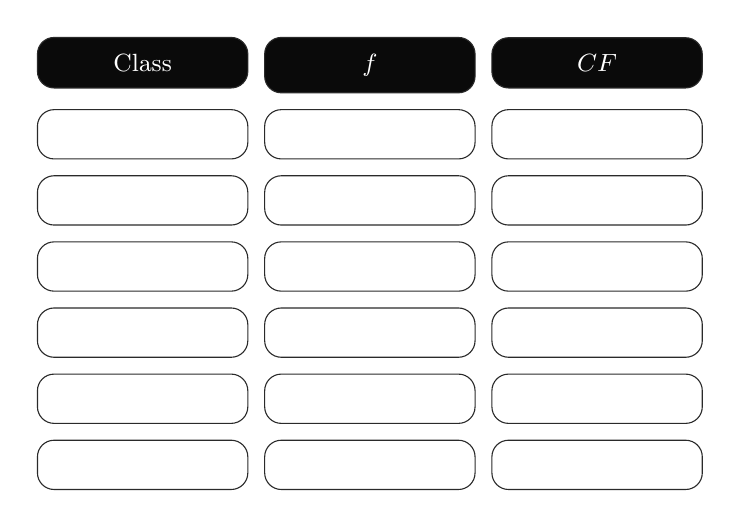
\begin{tikzpicture}
\matrix[matrix of nodes,
  nodes={draw=border, rounded corners=6pt, text width=2.25cm, align=center, font=\small, text=text, inner sep=6pt},
  row sep=2mm, column sep=2mm] (m) {
|[fill=solbg]| Class & |[fill=solbg]| $f$ & |[fill=solbg]| $CF$ \\
$41$--$50$ & $3$ & $3$ \\
$51$--$60$ & $17$ & $20$ \\
$61$--$70$ & $20$ & $40$ \\
$71$--$80$ & $30$ & $70$ \\
$81$--$90$ & $18$ & $88$ \\
$91$--$100$ & $2$ & $90$ \\
};
\end{tikzpicture}
\end{StepDiagram}
\EqDiagram{\(\displaystyle N=90\)}

\Step{2} Median: position \(N/2=45\) lies in class \(71\text{--}80\) (since \(CF\) goes \(40\to70\)).
Use boundaries \(70.5\) to \(80.5\) (\(h=10\)).
\EqDiagram{%
\[
\begin{aligned}
\text{Median} &= 70.5+\Big(\frac{45-40}{30}\Big)\,10\\
&= 70.5+1.6667\approx 72.17.
\end{aligned}
\]
}

\Step{3} Boys under the median \(\approx N/2\).
\EqDiagram{\(\displaystyle \#(\text{under median})=45\)}

\Step{4} First decile means first \(10\%\) of data \(\Rightarrow N/10=9\) boys.
\EqDiagram{\(\displaystyle \#(\text{first decile})=9\)}

\Step{5} 30th percentile means first \(30\%\) of data \(\Rightarrow 0.30\times 90=27\) boys.
\EqDiagram{\(\displaystyle \#(\text{in 30th percentile})=27\)}

\Step{6} “100th percentile” corresponds to the top end. From the table, the last class \(91\text{--}100\) has \(2\) boys.
\EqDiagram{\(\displaystyle \#(\text{top score group})=2\)}

\[
\boxed{
\begin{aligned}
&\text{(a) }90,\quad
\text{(b) median }\approx 72.17,\quad
\text{(c) }45,\\
&\text{(d) }9,\quad
\text{(e) }27,\quad
\text{(f) }2
\end{aligned}}
\]
\end{QAPair}

% ============================================================
% Q5
\begin{QAPair}{Question 5}
\textcolor{gold}{\bfseries Question:} Masses (kg) of 50 cubs:

\[
\begin{array}{c|cccccc}
\text{Mass (kg)} & 60\!-\!64 & 65\!-\!69 & 70\!-\!74 & 75\!-\!79 & 80\!-\!84 & 85\!-\!89\\ \hline
f & 2 & 6 & 12 & 14 & 10 & 6
\end{array}
\]

(i) Make cumulative frequency table.  
(ii) Make cumulative frequency polygon and estimate cubs above \(77\) kg.  
(iii) Make ogive and estimate cubs above \(77\) kg.  
(iv) Compare (ii) and (iii).
\tcblower
\textcolor{green}{\bfseries Answer:}\par

\Step{1} Cumulative frequency table (less-than type).
\begin{StepDiagram}
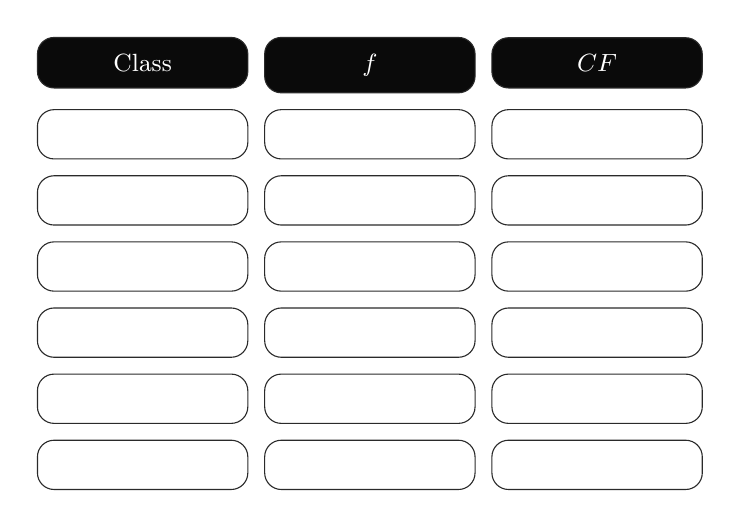
\begin{tikzpicture}
\matrix[matrix of nodes,
  nodes={draw=border, rounded corners=6pt, text width=2.25cm, align=center, font=\small, text=text, inner sep=6pt},
  row sep=2mm, column sep=2mm] (m) {
|[fill=solbg]| Class & |[fill=solbg]| $f$ & |[fill=solbg]| $CF$ \\
$60$--$64$ & $2$ & $2$ \\
$65$--$69$ & $6$ & $8$ \\
$70$--$74$ & $12$ & $20$ \\
$75$--$79$ & $14$ & $34$ \\
$80$--$84$ & $10$ & $44$ \\
$85$--$89$ & $6$ & $50$ \\
};
\end{tikzpicture}
\end{StepDiagram}
\EqDiagram{\(\displaystyle N=50\)}

\Step{2} Estimate \(CF(77)\) by linear interpolation in class \(75\text{--}79\).
Boundaries: \(74.5\) to \(79.5\) (\(h=5\)), class frequency \(f=14\).
\EqDiagram{%
\[
\begin{aligned}
CF(74.5)&=20,\\
77\ \text{is } \frac{77-74.5}{5}=0.5\ \text{of the class width} 
&\Rightarrow CF(77)\approx 20+14(0.5)=27,\\
\#(>77)&\approx 50-27=23.
\end{aligned}
\]
}

\Step{3} Ogive reading is very close to polygon reading, so the estimates match closely.
\EqDiagram{\(\displaystyle \#(>77)\approx 23\) cubs (by both methods).}

\[
\boxed{\text{Estimated cubs above }77\text{ kg} \approx 23\text{ (polygon and ogive agree).}}
\]
\end{QAPair}

% ============================================================
% Q6
\begin{QAPair}{Question 6}
\textcolor{gold}{\bfseries Question:} Study the cumulative curve (heights of 100 buildings) and find:
(a) buildings with height \(<50\) m,
(b) \% buildings higher than \(40\) m,
(c) ratio of buildings \(<50\) m to \(>50\) m,
(d) number of buildings in first quartile,
(e) maximum height under 8th decile,
(f) maximum height of buildings not falling under 30th percentile.
\tcblower
\textcolor{green}{\bfseries Answer:}\par

\Step{1} From the curve, \(CF(50)\approx 80\).
\EqDiagram{\(\displaystyle \text{(a) }\#(<50)\approx 80\)}

\Step{2} If \(CF(40)\approx 40\), then \(\#(>40)\approx 100-40=60\Rightarrow 60\%\).
\EqDiagram{\(\displaystyle \text{(b) }\%(\text{higher than }40)\approx 60\%\)}

\Step{3} Ratio:
\[
<50\approx 80,\quad >50\approx 20 \Rightarrow 80:20=4:1.
\]
\begin{StepDiagram}

\begin{tikzpicture}[scale=1.0]
\draw[base] (0,0) rectangle (6,0.8);
\draw[new] (0,0) rectangle (4.8,0.8);
\node[lab] at (2.4,0.4) {$<50$ m: 80};
\node[lab] at (5.4,0.4) {$>50$ m: 20};
\node[labm] at (3,-0.35) {ratio $80:20=4:1$};
\end{tikzpicture}
\end{StepDiagram}

\Step{4} First quartile contains first \(25\%\) of 100 buildings \(\Rightarrow 25\) buildings.
\EqDiagram{\(\displaystyle \text{(d) First quartile size}=25\text{ buildings}\)}

\Step{5} 8th decile is the 80th percentile: read height at \(CF=80\) (about \(50\) m).
\EqDiagram{\(\displaystyle \text{(e) }D_8 \approx 50\text{ m}\)}

\Step{6} 30th percentile corresponds to \(CF=30\) (about \(38\) m). Buildings not under \(P_{30}\) have height \(>38\) m; the maximum height is the top of the curve (about \(75\) m).
\EqDiagram{\(\displaystyle P_{30}\approx 38\text{ m}\ \Rightarrow\ \text{max among those above }P_{30}\approx 75\text{ m}\)}

\[
\boxed{
\begin{aligned}
&\text{(a) } \approx 80,\quad
\text{(b) } \approx 60\%,\quad
\text{(c) } \approx 4:1,\\
&\text{(d) }25,\quad
\text{(e) } \approx 50\text{ m},\quad
\text{(f) max }\approx 75\text{ m}
\end{aligned}}
\]
\end{QAPair}

% ============================================================
% Q7
\begin{QAPair}{Question 7}
\textcolor{gold}{\bfseries Question:} Mr. Rashid wants to analyze the salaries of his employees.
The first quartile \(Q_1=\text{Rs. }50{,}000\), the second quartile \(Q_2=\text{Rs. }70{,}000\),
the third quartile \(Q_3=\text{Rs. }90{,}000\) and the minimum and maximum salaries are
\(\text{Rs. }25{,}000\) and \(\text{Rs. }150{,}000\) respectively. Find range and interquartile range of the data.
\tcblower
\textcolor{green}{\bfseries Answer:}\par

\Step{1} Use the range formula.
\[
\text{Range}=\text{Max}-\text{Min}=150{,}000-25{,}000=125{,}000.
\]
\begin{StepDiagram}
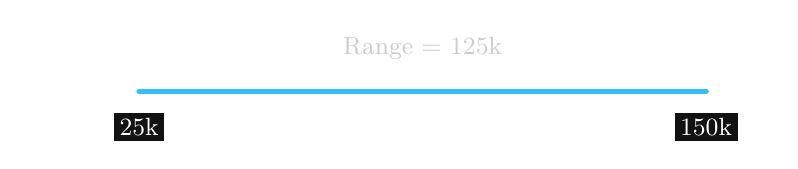
\begin{tikzpicture}[scale=1.0]
\draw[base, -{Stealth[length=3mm]}] (-0.2,0) -- (9.2,0);
\node[lab, fill=pairbg, inner sep=2pt] at (1.2,-0.45) {25k};
\node[lab, fill=pairbg, inner sep=2pt] at (8.4,-0.45) {150k};
\draw[new, line width=2pt] (1.2,0) -- (8.4,0);
\node[labm] at (4.8,0.55) {Range = 125k};
\end{tikzpicture}
\end{StepDiagram}

\Step{2} Use the interquartile range (IQR) formula.
\[
IQR=Q_3-Q_1=90{,}000-50{,}000=40{,}000.
\]
\begin{StepDiagram}
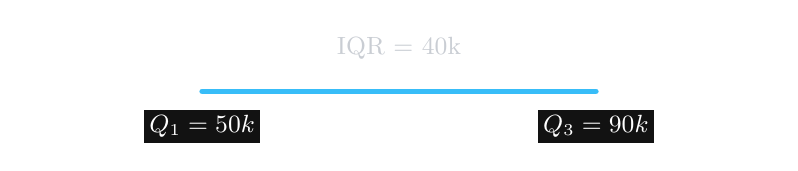
\begin{tikzpicture}[scale=1.0]
\draw[base, -{Stealth[length=3mm]}] (-0.2,0) -- (9.2,0);
\draw[base] (2,0.12)--(2,-0.12);
\draw[base] (7,0.12)--(7,-0.12);
\node[lab, fill=pairbg, inner sep=2pt] at (2,-0.45) {$Q_1=50k$};
\node[lab, fill=pairbg, inner sep=2pt] at (7,-0.45) {$Q_3=90k$};
\draw[new, line width=2pt] (2,0) -- (7,0);
\node[labm] at (4.5,0.55) {IQR = 40k};
\end{tikzpicture}
\end{StepDiagram}

\[
\boxed{\text{Range}=\text{Rs. }125{,}000,\qquad IQR=\text{Rs. }40{,}000.}
\]
\end{QAPair}

% ============================================================
% Q8
\begin{QAPair}{Question 8}
\textcolor{gold}{\bfseries Question:} Khadeeja scored \(85\) on a test, and the teacher reported that her score was in the \textbf{75th percentile}.
What does this information indicate about the status of Khadeeja in her class?
\tcblower
\textcolor{green}{\bfseries Answer:}\par

\Step{1} Interpret the 75th percentile.
\EqDiagram{Being in the \textbf{75th percentile} means Khadeeja scored \textbf{better than (or equal to) about 75\%} of the students.}

\Step{2} Convert that into class position.
\EqDiagram{So, she is in the \textbf{top 25\%} of the class, and only about \textbf{25\%} students scored higher than her.}

\begin{StepDiagram}

\begin{tikzpicture}[scale=1.0]
\draw[base] (0,0) rectangle (8,0.9);
\draw[new, line width=2pt] (0,0) -- (6,0); % 75% mark
\draw[help] (6,0) -- (6,0.9);
\node[lab] at (3,0.45) {75\% below her};
\node[lab] at (7,0.45) {top 25\%};
\node[labm] at (6,-0.35) {$P_{75}$};
\end{tikzpicture}
\end{StepDiagram}

\[
\boxed{\text{Khadeeja is among the top }25\%\text{ students in her class.}}
\]
\end{QAPair}

% ============================================================
% Q9
\begin{QAPair}{Question 9}
\textcolor{gold}{\bfseries Question:} Uzair wants to price his house based on the prices of similar houses in the area.
The prices have \(Q_1=\text{Rs. }20{,}000{,}000\), \(Q_2=\text{Rs. }25{,}000{,}000\), \(Q_3=\text{Rs. }30{,}000{,}000\),
and a maximum price of \(\text{Rs. }35{,}000{,}000\).
What is the possible price of the house if it is in the \textbf{third quartile}? Also find IQR of the data.
\tcblower
\textcolor{green}{\bfseries Answer:}\par

\Step{1} Meaning of “in the third quartile”.
\EqDiagram{The \textbf{third quartile region} is from \(Q_2\) to \(Q_3\) (i.e., the \textbf{50th to 75th percentile}).}

So a possible price is:
\[
25{,}000{,}000 \le \text{Price} \le 30{,}000{,}000.
\]

\begin{StepDiagram}
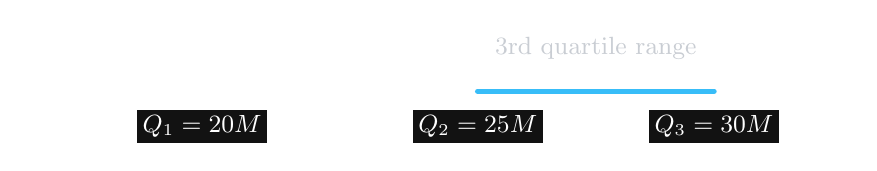
\begin{tikzpicture}[scale=1.0]
\draw[base, -{Stealth[length=3mm]}] (-0.2,0) -- (10.2,0);
\draw[base] (2,0.12)--(2,-0.12);
\draw[base] (5.5,0.12)--(5.5,-0.12);
\draw[base] (8.5,0.12)--(8.5,-0.12);
\node[lab, fill=pairbg, inner sep=2pt] at (2,-0.45) {$Q_1=20M$};
\node[lab, fill=pairbg, inner sep=2pt] at (5.5,-0.45) {$Q_2=25M$};
\node[lab, fill=pairbg, inner sep=2pt] at (8.5,-0.45) {$Q_3=30M$};
\draw[new, line width=2pt] (5.5,0) -- (8.5,0);
\node[labm] at (7.0,0.55) {3rd quartile range};
\end{tikzpicture}
\end{StepDiagram}

\Step{2} Interquartile range.
\[
IQR=Q_3-Q_1=30{,}000{,}000-20{,}000{,}000=10{,}000{,}000.
\]
\EqDiagram{\(\displaystyle IQR=\text{Rs. }10{,}000{,}000\)}

\[
\boxed{\text{Possible price: Rs. }25{,}000{,}000\text{ to Rs. }30{,}000{,}000;\quad IQR=\text{Rs. }10{,}000{,}000.}
\]
\end{QAPair}

% ============================================================
% Q10
\begin{QAPair}{Question 10}
\textcolor{gold}{\bfseries Question:} The adjoining cumulative frequency curve shows the number of faulty items in a shipment of \(100\) items produced by Khani's Collection.
Estimate:
(i) the median, (ii) lower quartile, (iii) upper quartile, (iv) IQR,
(v) 7th decile, (vi) 30th percentile.
\tcblower
\textcolor{green}{\bfseries Answer:}\par

\Step{1} Because \(N=100\), the key cumulative frequencies are:
\[
\begin{aligned}
Q_1 &: CF=25, \qquad \text{Median }(Q_2): CF=50,\\
Q_3 &: CF=75, \qquad D_7: CF=70, \qquad P_{30}: CF=30.
\end{aligned}
\]
\EqDiagram{On an ogive: draw a \textbf{horizontal line} at the required \(CF\), meet the curve, then drop a \textbf{vertical line} to the \(x\)-axis to read the value.}

\Step{2} Read \(Q_1, Q_2, Q_3\) from the curve (approx).
From the given curve:
\[
Q_1\approx 30,\quad \text{Median}\approx 35,\quad Q_3\approx 49\ \text{(faulty items)}.
\]

\begin{StepDiagram}
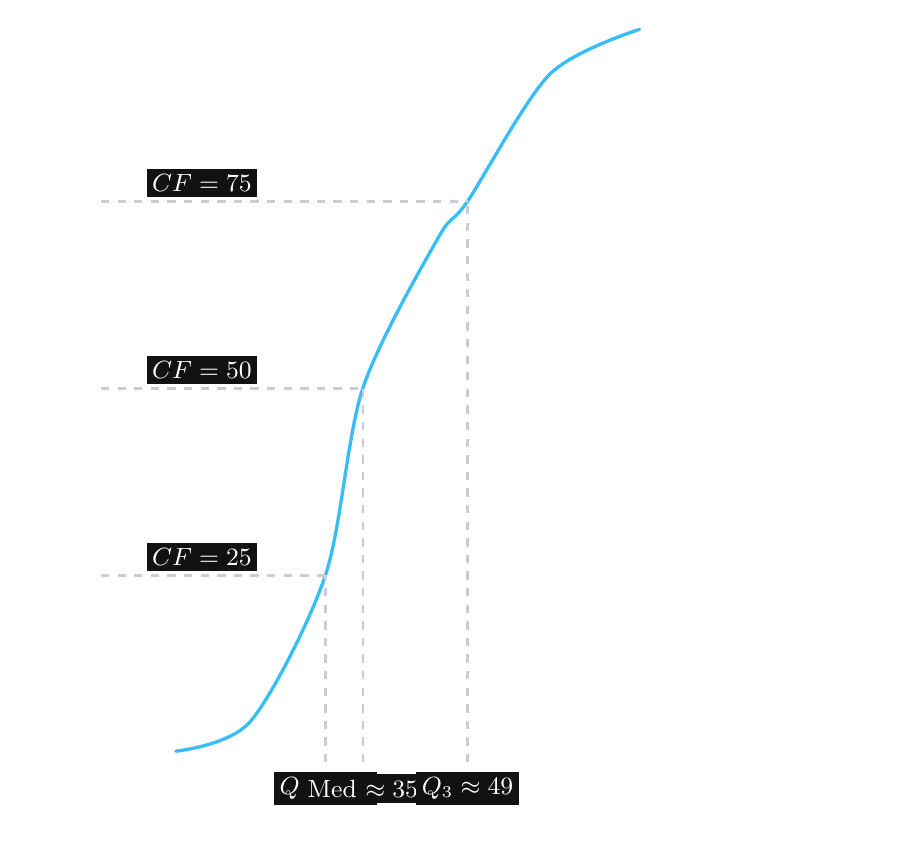
\begin{tikzpicture}[scale=0.95]
% axes
\draw[base, -{Stealth[length=3mm]}] (0,0) -- (9.2,0);
\draw[base, -{Stealth[length=3mm]}] (0,0) -- (0,6.2);
\node[lab] at (9.35,-0.15) {Faulty items};
\node[lab] at (-0.25,6.35) {CF};

% x ticks (10..80) mapped as 1..8
\foreach \x/\t in {1/10,2/20,3/30,4/40,5/50,6/60,7/70,8/80}{
  \draw[base] (\x,0.12)--(\x,-0.12);
  \node[lab] at (\x,-0.45) {\t};
}
% y ticks (20..100) mapped as 1..5
\foreach \y/\t in {1/20,2/40,3/60,4/80,5/100}{
  \draw[base] (0.12,\y)--(-0.12,\y);
  \node[lab] at (-0.6,\y) {\t};
}

% ogive curve (schematic)
\draw[new] plot[smooth] coordinates
  {(1.0,0.15) (2.0,0.55) (3.0,2.5) (3.5,5.0) (4.5,7.0) (4.9,7.5) (6.0,9.2) (7.2,9.8)};

% horizontals for Q1(25), Median(50), Q3(75) => y=2.5,5,7.5
\draw[help] (0,2.5) -- (3.0,2.5);
\draw[help] (0,5.0) -- (3.5,5.0);
\draw[help] (0,7.5) -- (4.9,7.5);
\draw[help] (3.0,0) -- (3.0,2.5);
\draw[help] (3.5,0) -- (3.5,5.0);
\draw[help] (4.9,0) -- (4.9,7.5);

\node[lab, fill=pairbg, inner sep=2pt] at (1.35,2.75) {$CF=25$};
\node[lab, fill=pairbg, inner sep=2pt] at (1.35,5.25) {$CF=50$};
\node[lab, fill=pairbg, inner sep=2pt] at (1.35,7.75) {$CF=75$};

\node[lab, fill=pairbg, inner sep=2pt] at (3.0,-0.35) {$Q_1\approx 30$};
\node[lab, fill=pairbg, inner sep=2pt] at (3.5,-0.35) {Med $\approx 35$};
\node[lab, fill=pairbg, inner sep=2pt] at (4.9,-0.35) {$Q_3\approx 49$};
\end{tikzpicture}
\end{StepDiagram}

\Step{3} Compute IQR.
\[
IQR\approx Q_3-Q_1\approx 49-30=19.
\]
\EqDiagram{\(\displaystyle IQR\approx 19\) faulty items}

\Step{4} Read 7th decile and 30th percentile from the curve (approx).
\[
D_7=P_{70}\approx 45,\qquad P_{30}\approx 31.
\]

\begin{StepDiagram}
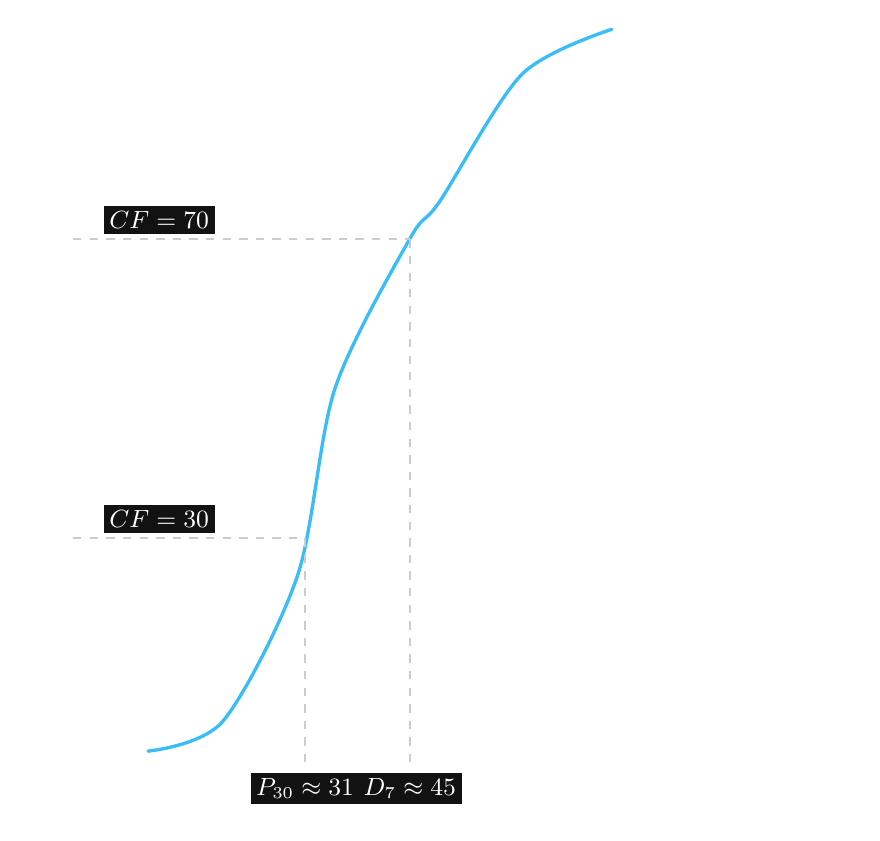
\begin{tikzpicture}[scale=0.95]
% axes
\draw[base, -{Stealth[length=3mm]}] (0,0) -- (9.2,0);
\draw[base, -{Stealth[length=3mm]}] (0,0) -- (0,6.2);
\node[lab] at (9.35,-0.15) {Faulty items};
\node[lab] at (-0.25,6.35) {CF};

% x ticks
\foreach \x/\t in {1/10,2/20,3/30,4/40,5/50,6/60,7/70,8/80}{
  \draw[base] (\x,0.12)--(\x,-0.12);
  \node[lab] at (\x,-0.45) {\t};
}

% curve (same schematic)
\draw[new] plot[smooth] coordinates
  {(1.0,0.15) (2.0,0.55) (3.0,2.5) (3.5,5.0) (4.5,7.0) (4.9,7.5) (6.0,9.2) (7.2,9.8)};

% P30: CF=30 => y=3.0, x≈3.1 (31)
\draw[help] (0,3.0) -- (3.1,3.0);
\draw[help] (3.1,0) -- (3.1,3.0);
\node[lab, fill=pairbg, inner sep=2pt] at (1.15,3.25) {$CF=30$};
\node[lab, fill=pairbg, inner sep=2pt] at (3.1,-0.35) {$P_{30}\approx 31$};

% D7: CF=70 => y=7.0, x≈4.5 (45)
\draw[help] (0,7.0) -- (4.5,7.0);
\draw[help] (4.5,0) -- (4.5,7.0);
\node[lab, fill=pairbg, inner sep=2pt] at (1.15,7.25) {$CF=70$};
\node[lab, fill=pairbg, inner sep=2pt] at (4.5,-0.35) {$D_7\approx 45$};
\end{tikzpicture}
\end{StepDiagram}

\[
\boxed{
\begin{aligned}
&\text{Median }(Q_2)\approx 35,\quad
Q_1\approx 30,\quad
Q_3\approx 49,\\
&IQR\approx 19,\quad
D_7\approx 45,\quad
P_{30}\approx 31
\end{aligned}}
\]
\end{QAPair}

\end{document}
